
\subsection{Background}
    \textit{Satisfiability Modulo Theories (SMT)} is the problem of determining whether a
    mathematical formula is satisfiable. It generalizes the Boolean satisfiability problem (SAT) to
    more complex formulas involving real numbers, integers, and/or various data structures such as 
    lists, arrays, bit vectors, and strings.

% % % % % % % % % % % % % % % % % % % % % % % % % % % % % % % % % % % % % % % % % % % % % % % % % %

\subsection{Formulation} \label{subsec:SMT_formulation}
    In order to write a proper SMT formulation, we started from the SAT formulation (available in
    the Section \ref{chapter:SAT}) and we have replaced each boolean representation of integer 
    operators with the operators themself.\\

    In particular, the following replacements have been done:
    \begin{align*}
      \text{SMT} \ &\ \leftarrow\ \text{SAT}      \\
                 \cline{1-2}
        a \geq 1 \ &\ \leftarrow\ \text{at\_least\_one}(a) \\
        a \leq 1 \ &\ \leftarrow\ \text{at\_most\_one}(a)  \\
           a = 1 \ &\ \leftarrow\ \text{exactly\_one}(a)   \\
           a = b \ &\ \leftarrow\ \text{equal}(a,b)        \\
           a < b \ &\ \leftarrow\ lt(a,b)                  \\
        a \leq b \ &\ \leftarrow\ lte(a,b)                 \\
           a > b \ &\ \leftarrow\ gt(a,b)                  \\
        a \geq b \ &\ \leftarrow\ gte(a,b)                 \\
           a + b \ &\ \leftarrow\ sum\_b(a,b)              \\   
           a - b \ &\ \leftarrow\ sub\_b(a,b)                 
    \end{align*}

    The final formulation obtained is very "near" to the one defined for CP in the
    Section \ref{chapter:CP}.

% % % % % % % % % % % % % % % % % % % % % % % % % % % % % % % % % % % % % % % % % % % % % % % % % %

\subsection{Results}\label{subsec:SMT_results}
    All the experiments for the SMT technology have been executed on a laptop computer running 
    \texttt{macOS Monterey 12.3} equipped with the following hardware:
    \texttt{Apple M1 Pro 10-core, 16Gb Ram LPDDR5}.\\


    The results obtained for the \(Base\) Model, presented in the Figures 
    [\ref{fig:SMT_results_base1},\ref{fig:SMT_results_base2}], are in line with those obtained 
    previously in SAT (Section \ref{subsec:SAT_results}).\\

    \begin{figure}[H]
      \centering
      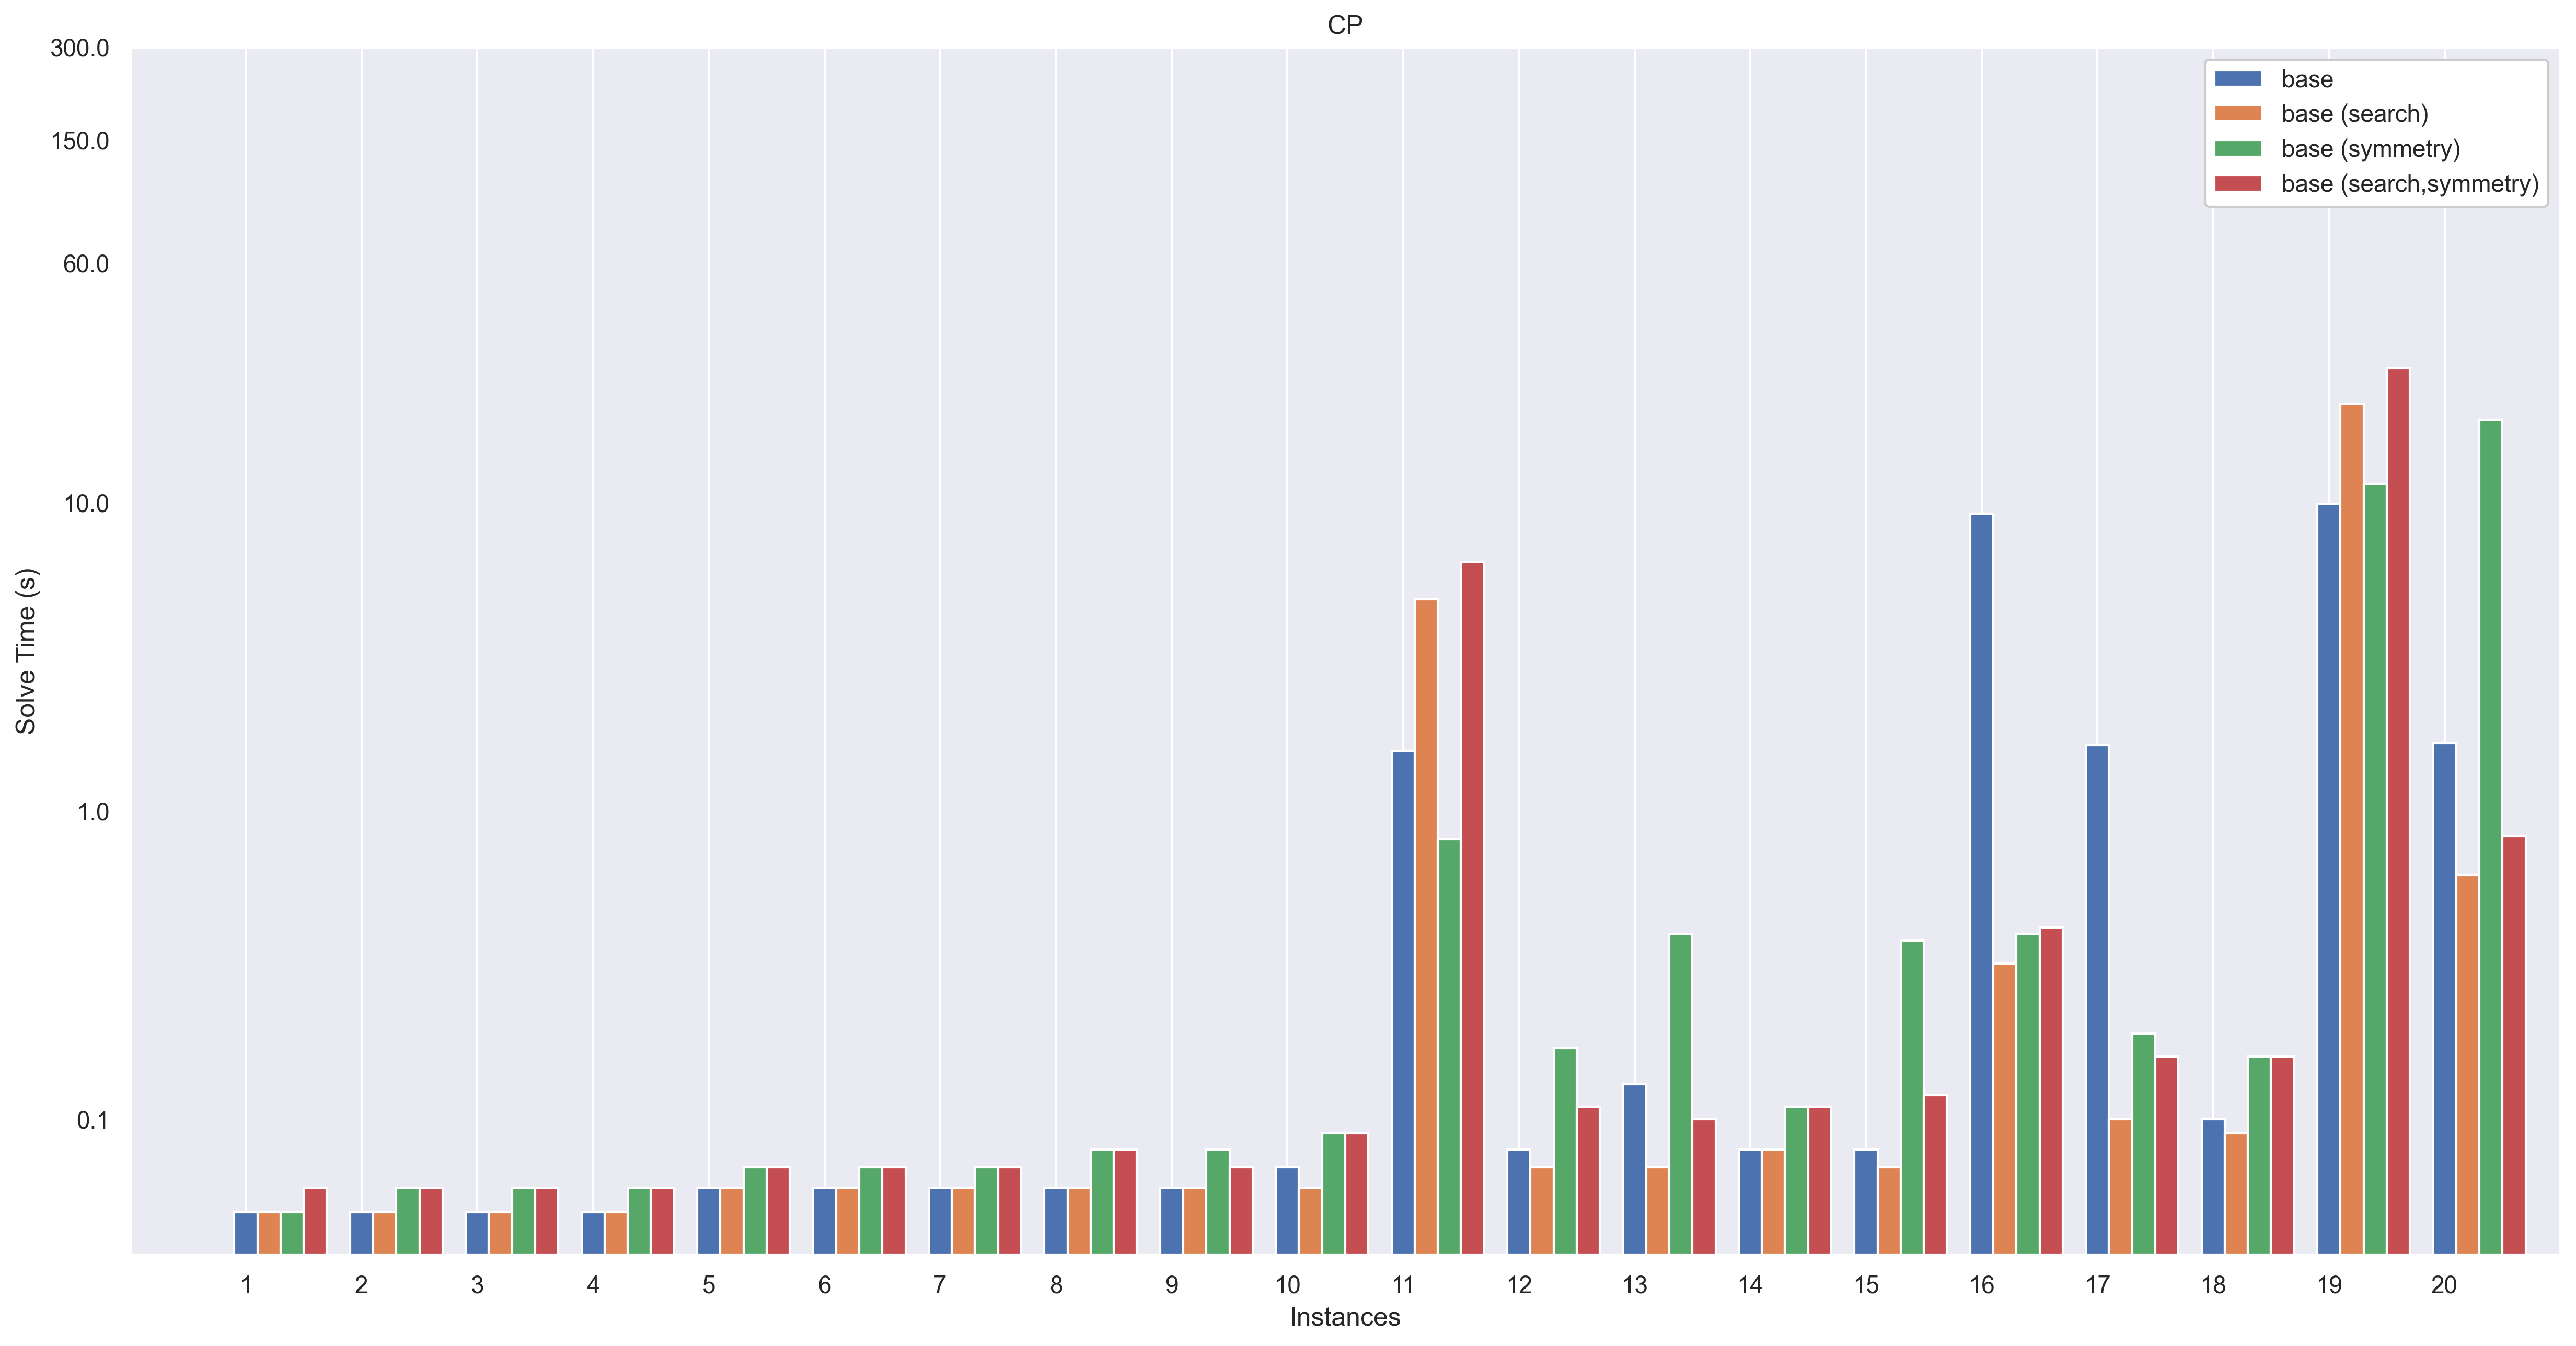
\includegraphics[width=1\textwidth]{05/results/base1.png}
      \caption{SMT \(Base\) Model: instances [1,20]}
      \label{fig:SMT_results_base1}
    \end{figure}
    \begin{figure}[H]
      \centering
      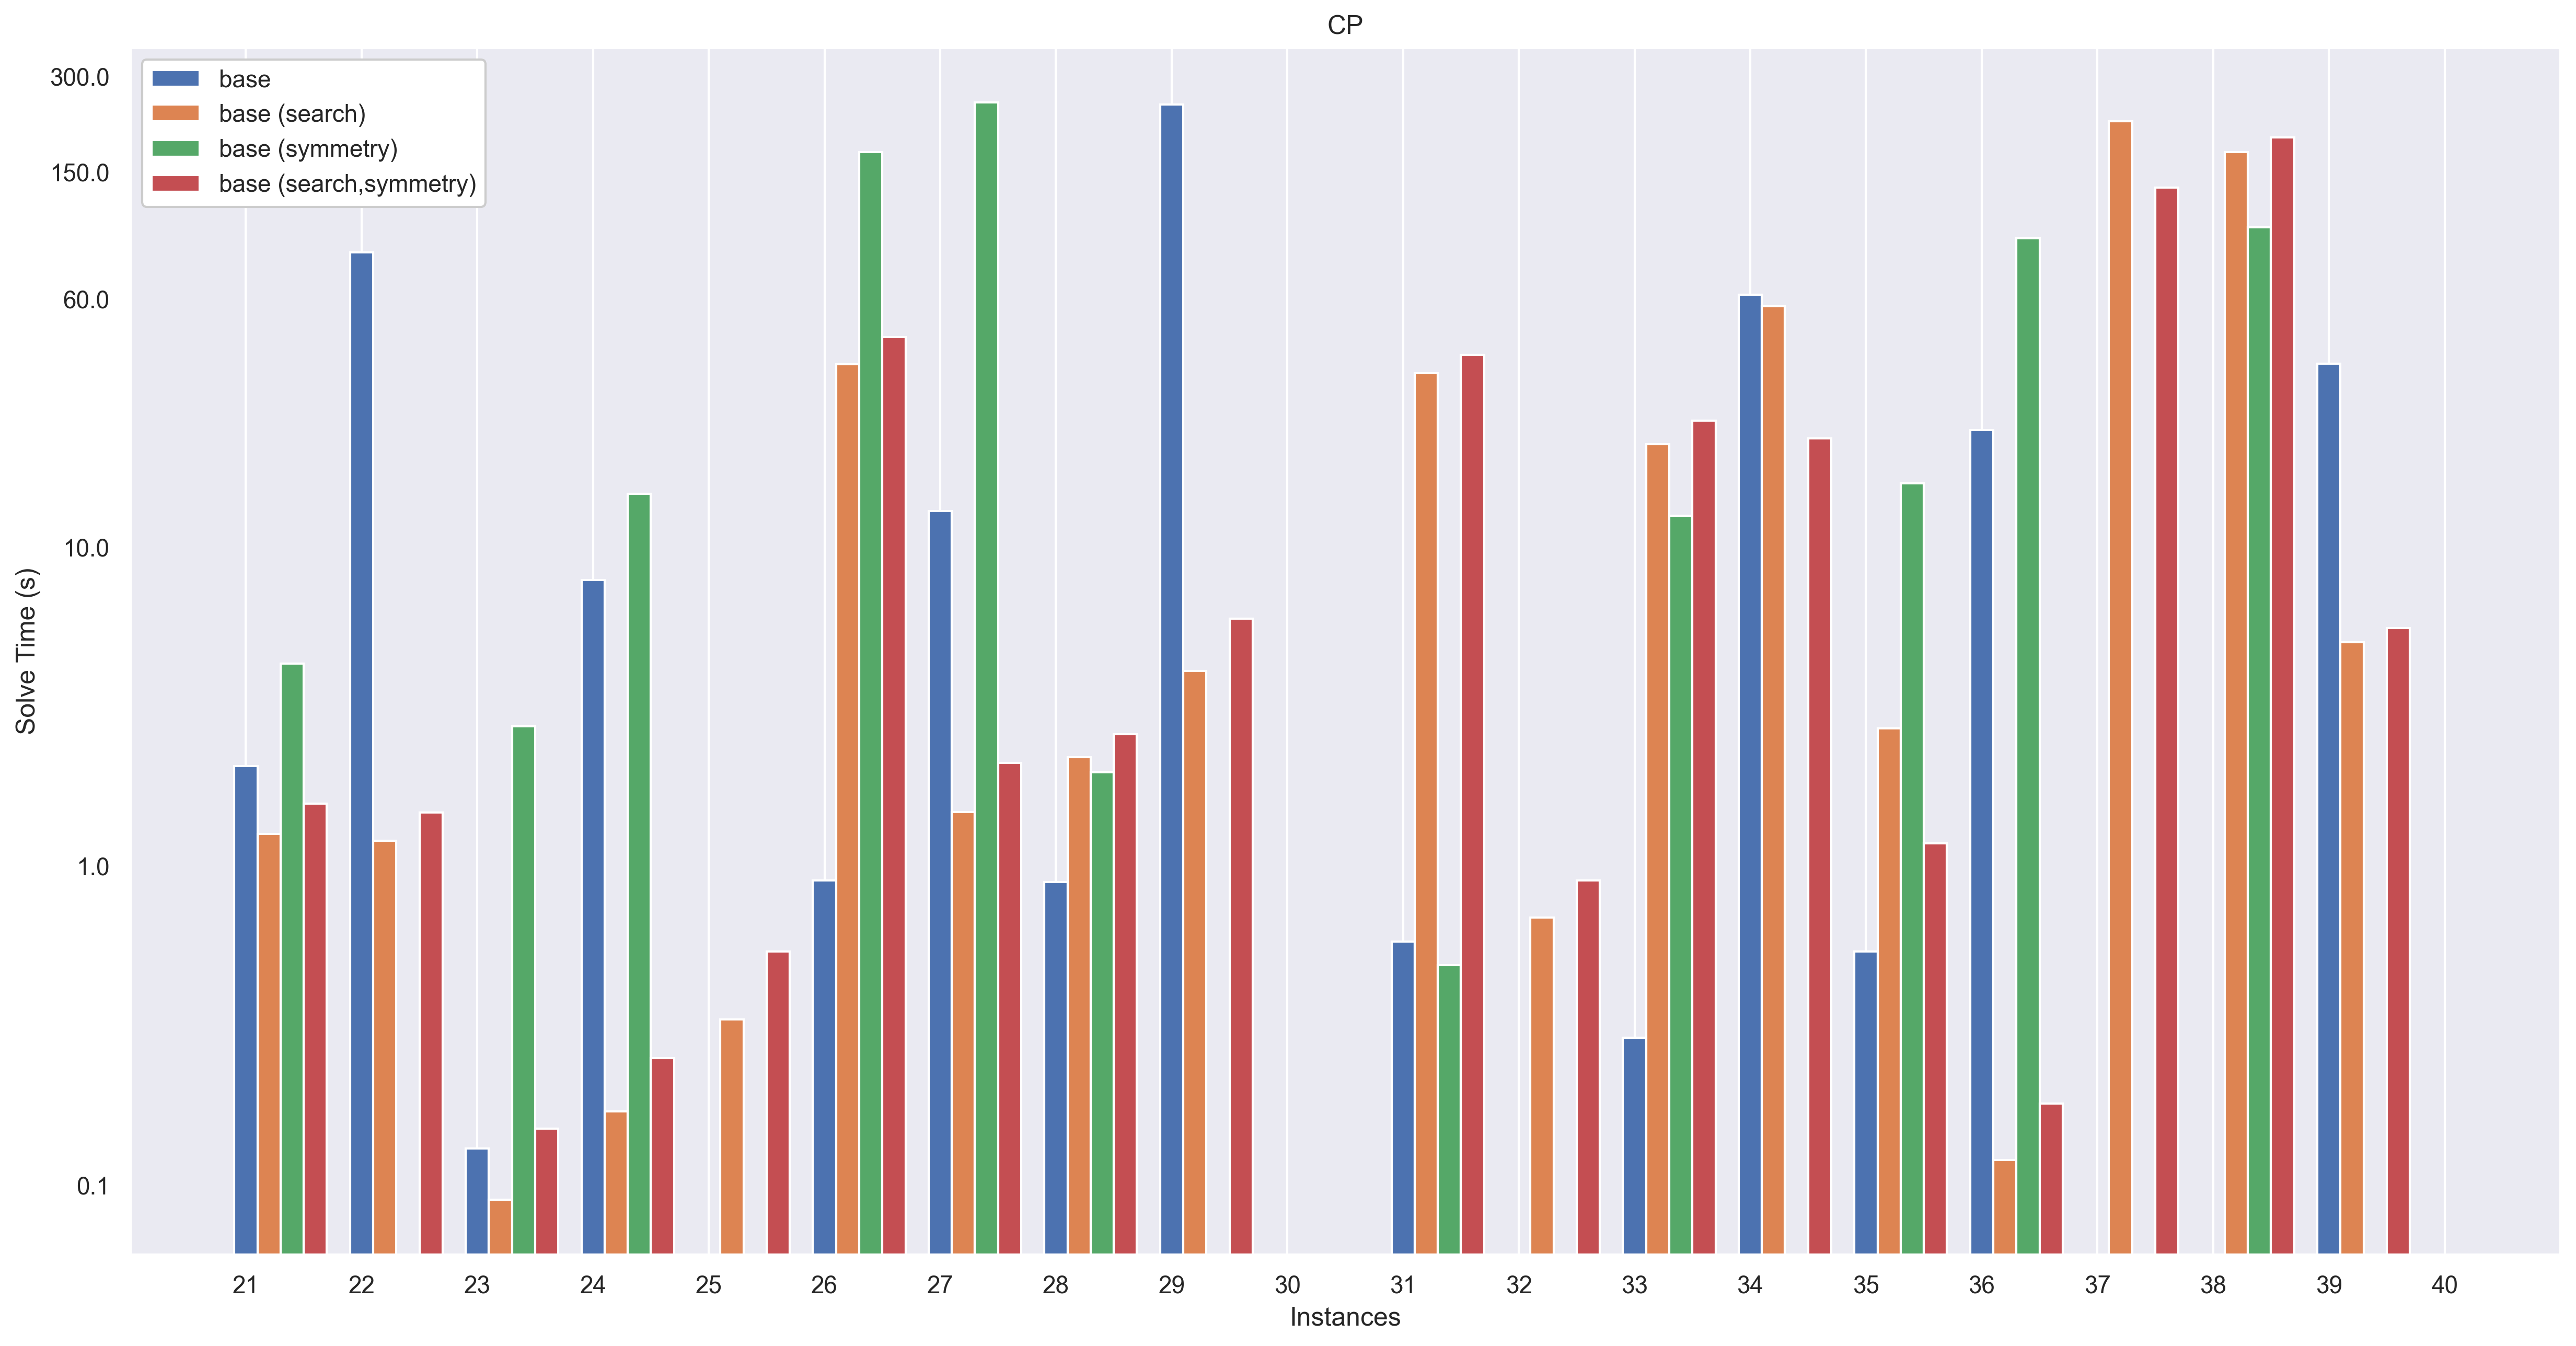
\includegraphics[width=1\textwidth]{05/results/base2.png}
      \caption{SMT \(Base\) Model: instances [21,40]}
      \label{fig:SMT_results_base2}
    \end{figure}

    The results obtained for the \(Rotation\) Model, presented in the Figures 
    [\ref{fig:SMT_results_rotation1},\ref{fig:SMT_results_rotation2}], are "slightly" better with 
    those obtained previously in SAT (Section \ref{subsec:SAT_results}). The latter statement 
    refers, in particular, to the average solve time needed for solve the same instances. Despite 
    this, as for the \(base\) Model, the total number of instances correctly solved haven't changed too much.\\

    \begin{figure}[H]
      \centering
      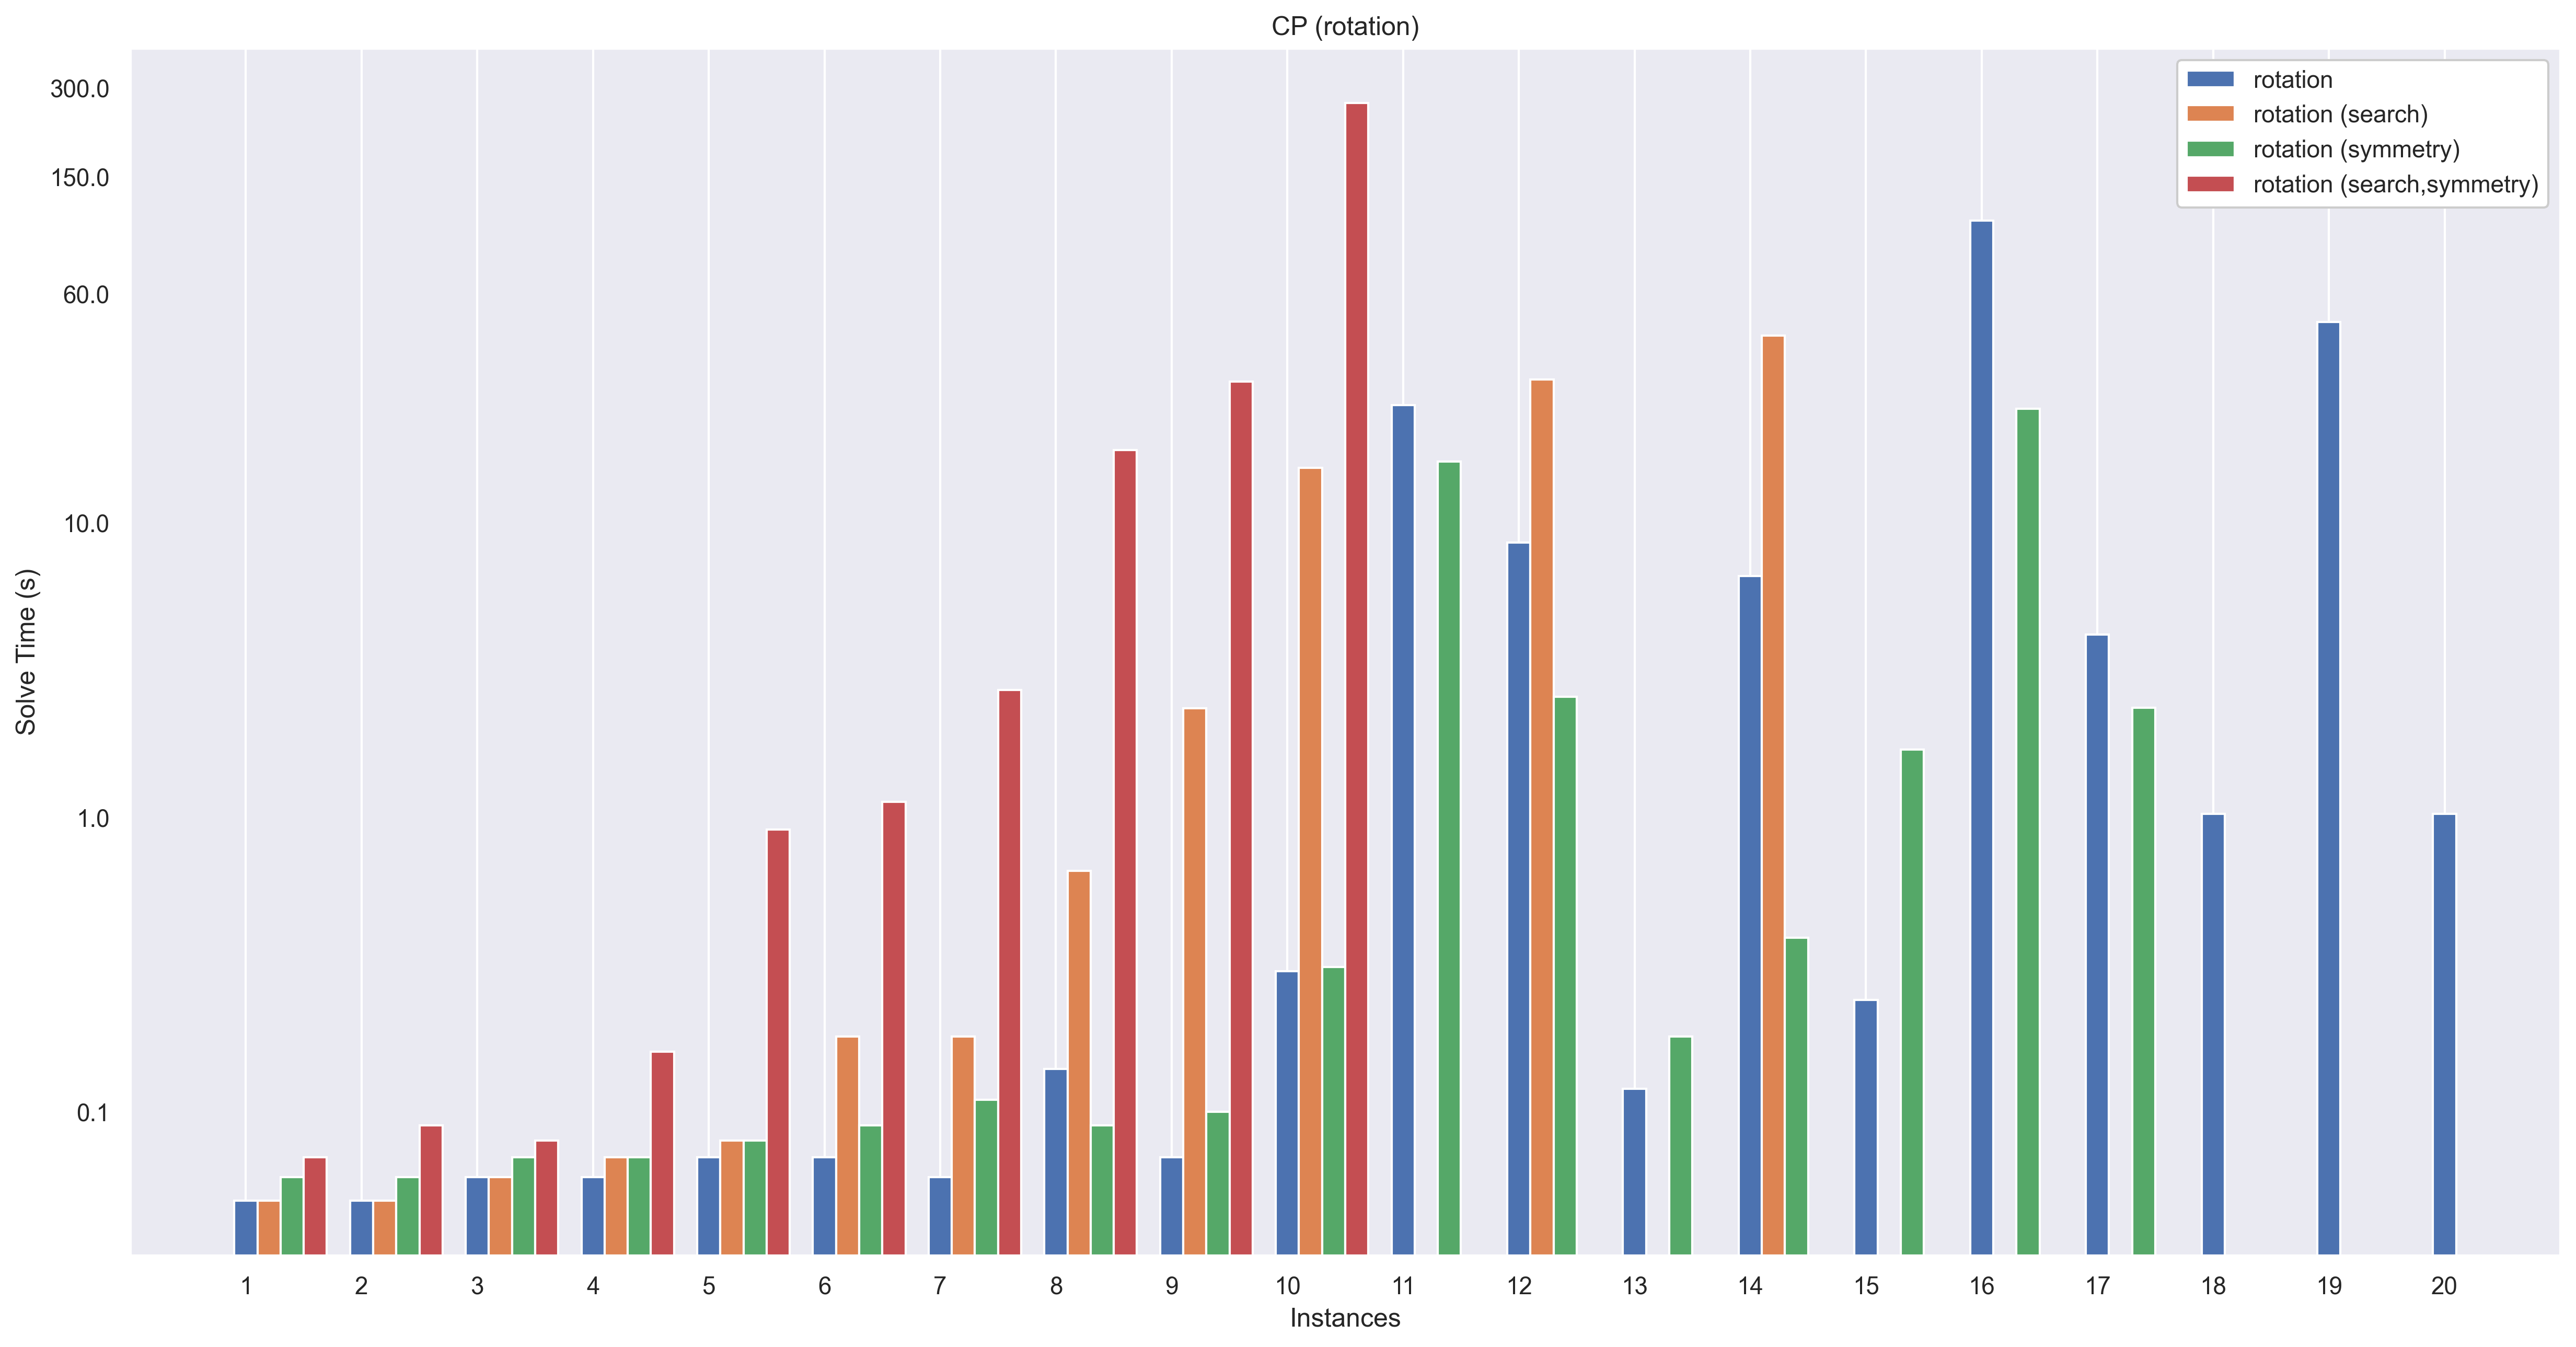
\includegraphics[width=1\textwidth]{05/results/rotation1.png}
      \caption{SMT \(Rotation\) Model: instances [1,20]}
      \label{fig:SMT_results_rotation1}
    \end{figure}
    \begin{figure}[H]
      \centering
      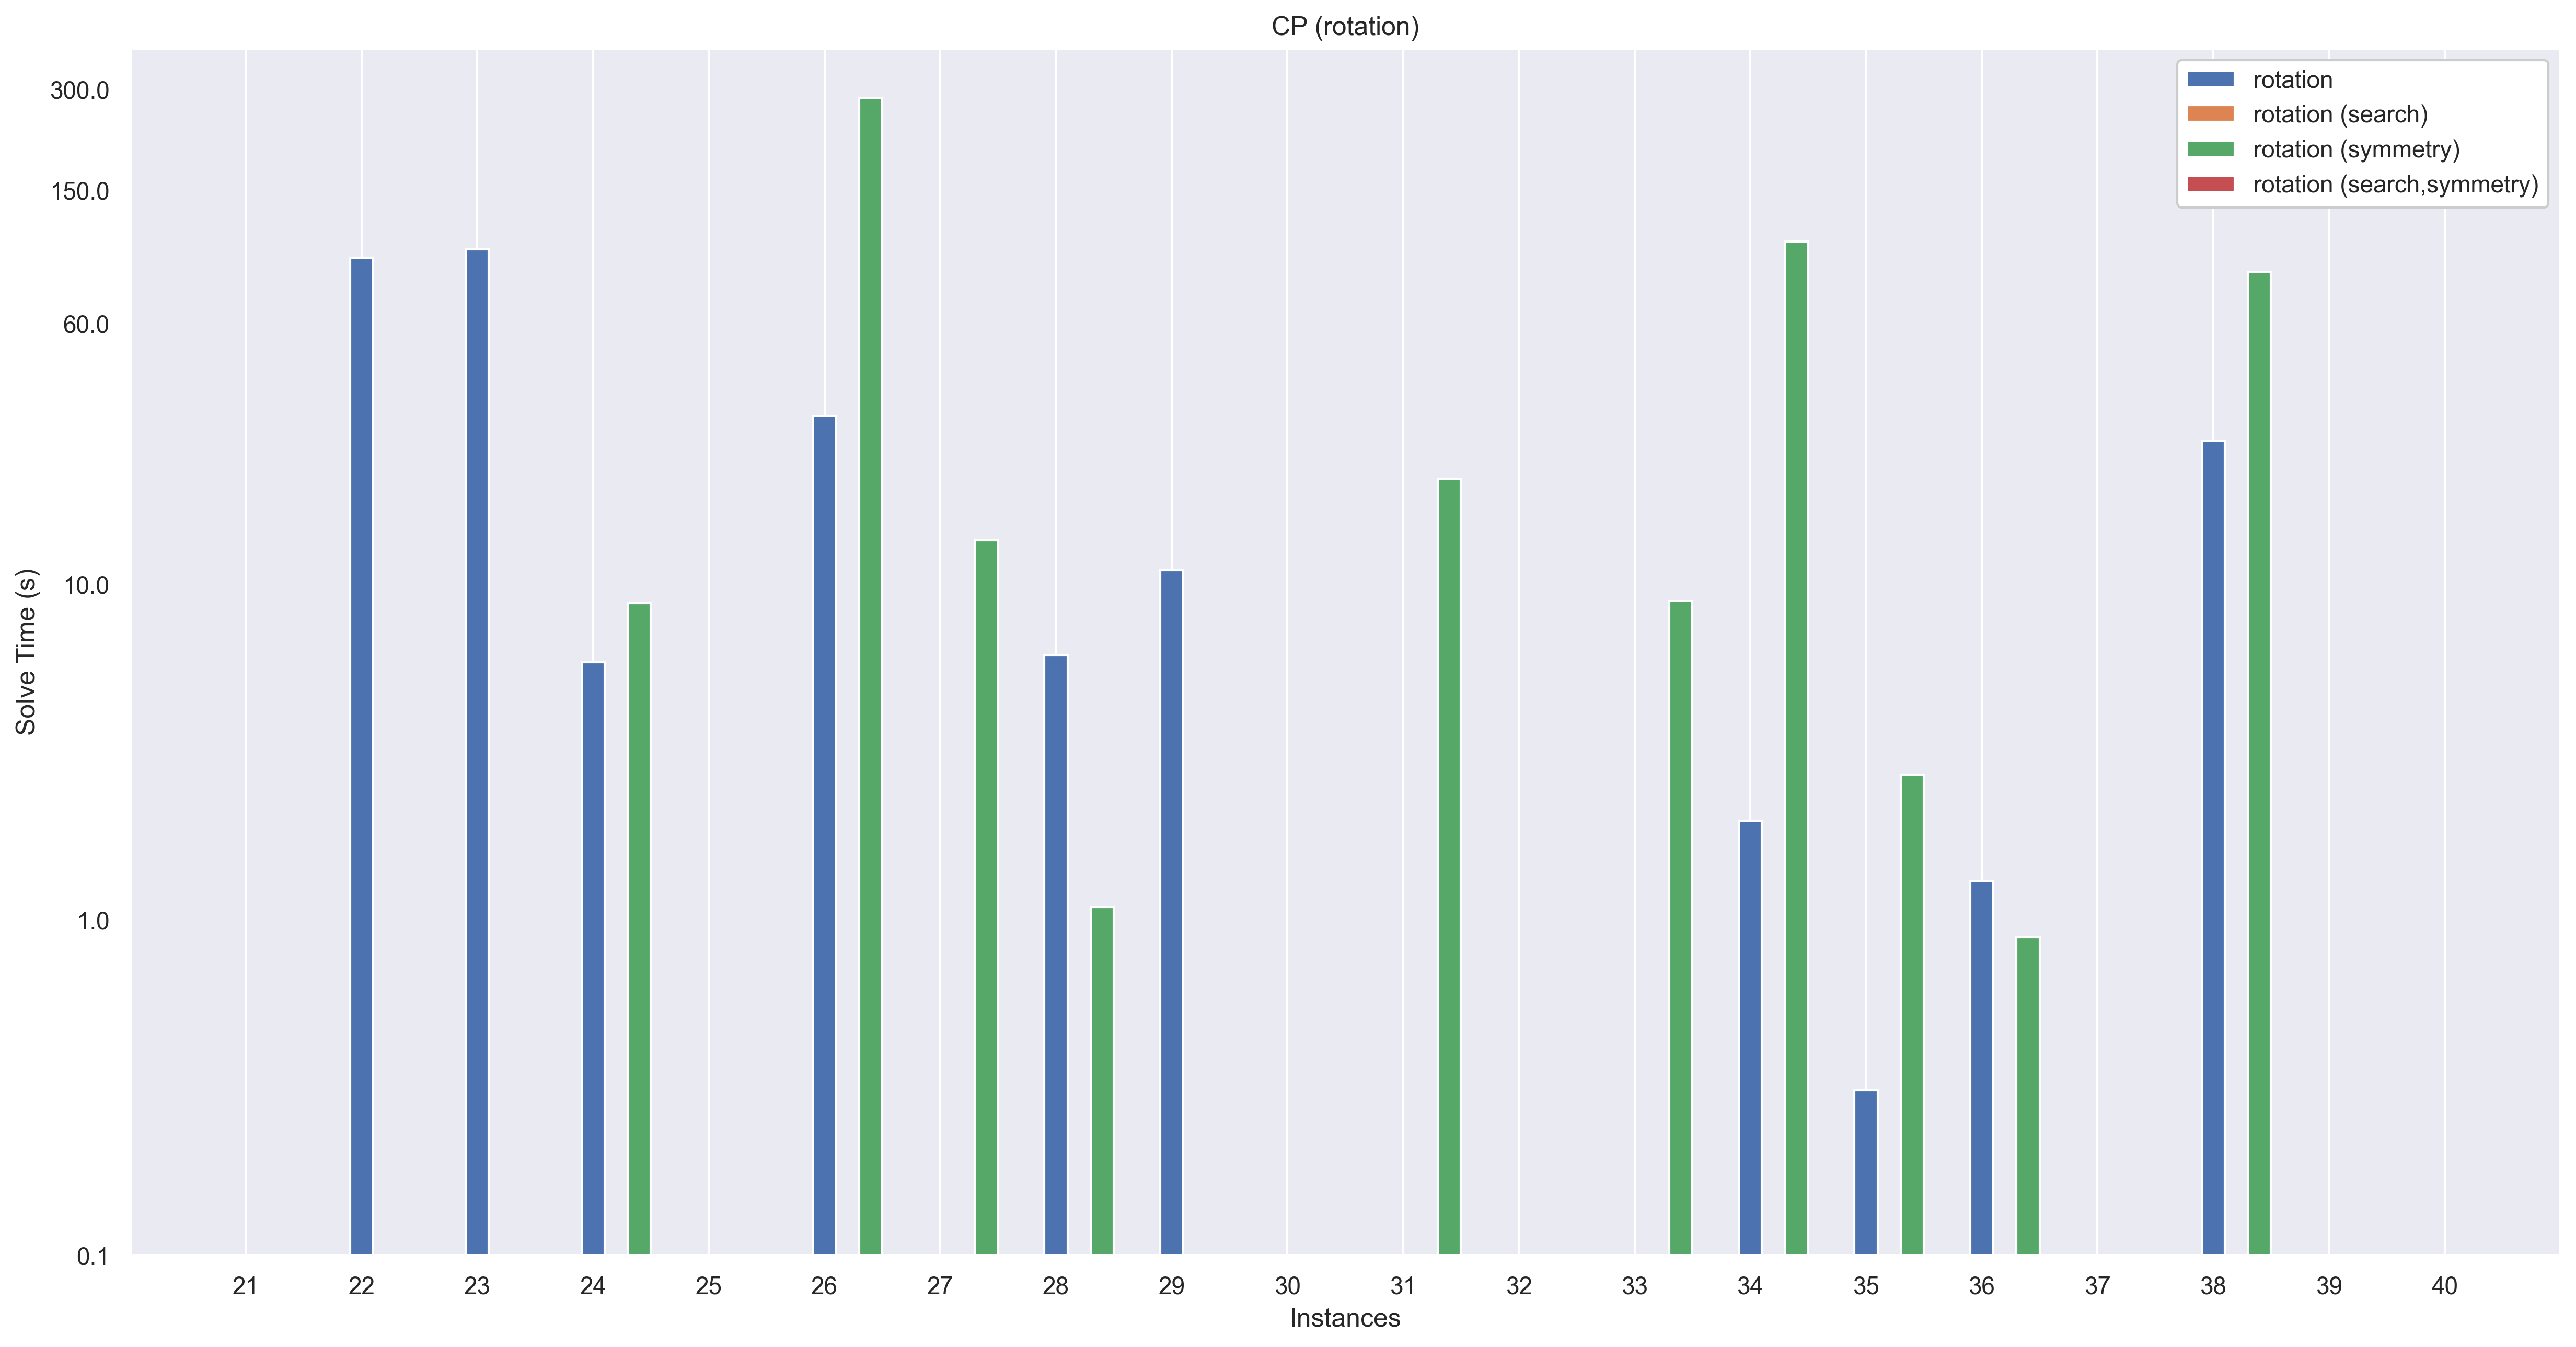
\includegraphics[width=1\textwidth]{05/results/rotation2.png}
      \caption{SMT \(Rotation\) Model: instances [21,40]}
      \label{fig:SMT_results_rotation2}
    \end{figure}

    Considerig the fact that SMT is an extension of SAT, we can see how similar are the results for
    these two technologies (SAT results are available in Section \ref{subsec:SAT_results}) when we 
    inspect the total number of correctly solved instances. \\

    Finally, through the similarity between the results of SAT and SMT, we have also showed the 
    validity of the conversion between the two formalizations 
    (SAT: Section \ref{subsec:SAT_predicates}, SMT: Section \ref{subsec:SMT_formulation}).
